\documentclass[12pt,a4paper,oneside,dvipsnames,table,svgnames,skins,theorems]{report}
\usepackage{ProfCollege}
\usepackage{tmbase} %pour le moment placé dans la racine du .tex ... !


\graphicspath{{C:/Users/Thom/Documents/latex nas/images/}} %chemin du fichier image
%\graphicspath{{C:/Users/Thomas/latex nas/images/}} %chemin du fichier image

\ordi{fixe} %pour fichier image
\matierechap{m} %m pour maths, pc pour physique chimie, rien pour vierge
\version{1} %1 : PROF   2: ELEVE sans corrigé  3: corrigé des exos sans le cours
\setcounter{chapter}{3} %compteur de chapitre

\begin{document}




\ifsectioncours


\chapter{Logarithme décimal}
\setcounter{page}{1}
\vspace{-0.5cm}
\section{Activité d'introduction}

On se propose de représenter sur un repère les masses de quelques animaux :

\begin{center}

\includegraphics[scale=0.7]{massemouche.png}\hspace{0.2cm}\includegraphics[scale=0.75]{massebaleine.png}
\vspace{0.1cm}

\includegraphics[scale=0.8]{massecheval.png}\hspace{0.2cm}\includegraphics[scale=0.75]{massechat.png}

\vspace{1cm}

\begin{tikzpicture}[yscale=1.5]

\draw[gray](-1.5,0)grid(10.5,0);
\draw[-stealth]|-(10.5,0)node[above]{$x$ (\si{\kilo\gram})};
\foreach \x in {-1,...,10} \draw (\x,-.1)node[below]{\x} -- (\x,0);


\end{tikzpicture}
\end{center}

\vspace{0.5cm}

Quel est le problème rencontré ? Quelle solution pour le contourner ? 
\vspace{0.1cm}

\pointilles{1}{}

\newpage

On propose un deuxième repère :

\begin{center}
\begin{tikzpicture}[scale=1.5]

\tkzInit[xmin=0, xmax=10000, xstep=1000]
\tkzDrawX
\tikzset{xlabel style/.append style={rotate=-30}}
\tkzLabelX[below right=3 pt, inner sep = 1pt]

\end{tikzpicture}
\end{center}

\vspace{0.5cm}

Cette échelle convient-elle pour placer tous les éléments ?
\vspace{0.1cm}

\pointilles{2}{}


Est-elle très satisfaisante ? \textbf{Expliquer} la réponse.
\vspace{0.1cm}

\pointilles{4}{}

\vspace{0.5cm}

\cadre{\pointilless{2}{Conclusion : }}

\vspace{0.5cm}

Il y a quelques années (avant l'invention de la calculatrice !) les scientifiques se sont heurtés à des difficultés similaires quand ils essayaient de faire des calculs compliqués, de comparer des éléments de tailles très différentes ... Ils ont élaboré des solutions pour traiter ce genre de situations.

\vspace{0.3cm}

\textbf{Donner} pour chaque animal sa masse exprimée sous la forme d'une puissance de 10 :
\vspace{0.5cm}

\begin{itemize}
\item Cheval : \lpointilles{5cm}
\item Chat : \lpointilles{5cm}
\item Baleine : \lpointilles{5cm}
\item Mouche : \lpointilles{5cm}
\end{itemize}
\vspace{0.5cm}

\textbf{Proposer} un placement des animaux en les classant par masse sur le repère en utilisant les résultats précédents :
\vspace{0.5cm}

\begin{center}
\begin{tikzpicture}[scale=1]

\tkzInit[xmin=-5, xmax=10, xstep=1]
\tkzDrawX
%\tikzset{xlabel style/.append style={rotate=-30}}
\tkzLabelX[below=3 pt]

\end{tikzpicture}
\end{center}

\newpage

\section{Le logarithme décimal}

Le logarithme décimal est un extracteur de puissance de 10. 
\vspace{0.1cm}

Il se note $\log$ et se dit "logarithme de base 10" (il y en a d'autres) et on a : 
\begin{large}
\begin{itemize}
\item $\log(10^4) = 4$
\item $\log(10^5) = 5$
\item $\log(10^8) =$ .........
\item $\log(10^{11}) =$ .........

\item $\log(1) =$ .........
\item $\log(10) = $ .........




\end{itemize}
\end{large}


\vspace{0.5cm}

\cadre{
\textbf{Nouvelle fonction : }
\vspace{0.5cm}

On appelle logarithme décimal (ou log base 10) la fonction :
\begin{itemize}
\item Définie sur $]0;+\infty[$
\item $f(x)= \log x$
\item elle s'annule pour $x=1$ (on a $\log 1=0$)
\end{itemize}
}

\begin{center}
\begin{tikzpicture}[scale=2]
\tkzInit[xmin=-2,xmax=12,ymin=-2,ymax=2,xstep=2]
\tkzGrid
\tkzAxeXY
\tkzSetUpPoint[size=6]
\tkzFct[color=red,domain=-1:11]{log10(\x)}
\tkzText(11,1.5){$\log (x)$}
\tkzDefPoint(1,0){A}  \tkzDrawPoint(A) \tkzLabelPoint(A){$A$}
\tkzDefPoint(10,1){B} \tkzDrawPoint(B) \tkzLabelPoint(B){$B$}
\end{tikzpicture}
\end{center}

\newpage

\section{Activité : Acoustique et Éclairement}

On retrouve des logarithmes décimaux quand les échelles des mesures s'étendent du très petit au très grand c'est le cas dans deux domaines de la physique (entre autre) : 
\begin{itemize}
\item L'acoustique
\item L'éclairement
\end{itemize}
Dans cette activité nous allons étudier quelques paramètres pour l'éclairement.
\vspace{0.5cm}

Notre oeil est un outil formidable qui s'adapte à l'éclairement et qui est sensible pour des valeurs allant de \SI{0.01}{\lux} (lumière de la lune en pleine nuit) à \SI{100000}{\lux} (la lumière en plein soleil par exemple). Le \si{\lux} est l'unité de l'éclairement et s'obtient avec un luxmètre :

\begin{center}
\includegraphics[scale=0.45]{luxmetre.png}
\end{center}

\textbf{Quelques questions} :

\begin{enumerate}
\item Quelle serait la longueur théorique de l'axe permettant de représenter l'échelle d'éclairement visible par l'oeil si on prenait $\SI{1}{\centi\meter} = \SI{1}{\lux} $ ? 
\item Serait-il possible de bien distinguer, sur cet axe, la limite basse ?
\item Proposer une méthode pour représenter sur une même échelle et de manière visible ces différents éclairements.
\item Représenter cette échelle.
\end{enumerate}

On pourra s'aider du tableau suivant :
\vspace{0.1cm}

\renewcommand{\arraystretch}{3}
\begin{tabularx}{\textwidth}{|C|C|C|C|C|C|C|C|C|}
\hline
{\footnotesize Éclairement} (\si{\lux}) & 0.01 & 0.1 & 1 & 10  & 100 & 1000 & 10000 &100000 \crh
E (\si{\lux}) puissance de 10 & & & & & $10^2$ & & &  \crh
$\log E$ & & & & & & & &  \crh

\end{tabularx}

\begin{enumerate}[resume]
\item Un court de tennis doit avoir un éclairement minimal de \SI{500}{\lux}. Placer cet éclairement sur l'axe.
\item Une tribune extérieure d'un stade doit avoir un éclairement proche de \SI{10}{\lux}. Placer cette valeur sur l'axe ainsi formé.
\end{enumerate}


\newpage

\section{Propriétés du logarithme}

Ces propriétés resteront vraies pour les autres logarithmes vus cette année et sont à savoir utiliser!

\vspace{0.5cm}

\begin{large}
\cadre{ Soient $a>0$ et $b>0$ deux nombres :
\vspace{0.5cm}

\begin{itemize}
\item $\log(a\times b) = \log a + \log b$ (transformation d'un produit en somme)
\item $\log \dfrac{a}{b} = \log a - \log b$ (transformation d'une division en soustraction)
\item $\log\dfrac{1}{b} = - \log b$ 
\item $\log 10 ^x = x $ ou encore $  10^{\log(x)} = x $
\item $\log a^n = n \log a $
\item $\log 1 = 0$ et $\log 10 = 1$

\end{itemize}
}
\end{large}

\vspace{0.5cm}

Exemples :
\begin{itemize}
\item $\log(5\times7) = \log 5 + \log 7$
\item $\log 90 = \log 9\times 10 = \log 9 + \log 10 = \log 9 = \log 3 \times 3 = \log 3 + \log 3 = 2\log 3$
\end{itemize}

\vspace{1cm}

\textbf{Activité facultative} : vérification des propriétés à l'aide d'un tableur
\vspace{0.5cm}

Travail à destination des plus rapides ou des plus motivés avec pour objectif de prendre en main le tableur et de vérifier les formules ci-dessus.
\begin{center}
\includegraphics[scale=0.75]{alealog.png}
\end{center}

La formule rentrée dans la case A2 est :  \mybox{=ALEA.ENTRE.BORNES(0;1000)} et elle permet de générer un nombre aléatoire entre 0 et 1000. Si votre tableur ne reconnait pas cette formule on peut écrire : \mybox{=ALEA()*1000} à la place.
\vspace{0.5cm}

\textbf{Travail} : reproduire cette feuille de calcul, générer aléatoirement en étirant la formule 10 valeurs de $a$ et $b$ et calculer les résultats dans les colonnes C à H et conclure.


\fi
\ifsectionexos
\newpage

\section{Exercices}
\Opensolutionfile{mycor}[ficcorex]

\exo{} Calculer les valeurs décimales arrondies au dixième des nombres :
\begin{itemize}
\item $\log 10^{-12}$
\item $\log 80$
\item $\log 1$
\item $\log 5$
\end{itemize}

\begin{correction}
\begin{itemize}
\item $\log 10^{-12} = -12$
\item $\log 80 = \log 8 = 0.9 $
\item $\log 1 = 0$
\item $\log 5 = 0.7$
\end{itemize}
\end{correction}

\finexo
\vspace{0.5cm}

\exo{} Compléter le tableau :
\vspace{0.1cm}

\renewcommand{\arraystretch}{2}
\begin{tabularx}{\textwidth}{|C|C|C|C|C|C|C|C|}
\hline
x & 1 & 2 & 4 & 8 & 16 & 32 & 64 \crh
$\log x$ & & & & & & &   \crh


\end{tabularx}
\begin{enumerate}
\item Donner la nature de la suite formée par la première ligne
\item Donner la nature de la suite formée par la deuxième ligne
\item Donner la raison de la première suite
\item Donner la raison de la deuxième suite
\item Calculer le $\log$ de la raison de la première suite. Que remarquez vous ?
\end{enumerate}


\begin{correction} Tableau : \\
\begin{tabularx}{\textwidth}{|C|C|C|C|C|C|C|C|}
\hline
x & 1 & 2 & 4 & 8 & 16 & 32 & 64 \crh
$\log x$ & 0 &  0.30 & 0.60 & 0.90 & 1.2 & 1.5 & 1.8    \crh

\end{tabularx}
\begin{enumerate}
\item géométrique
\item arithmétique
\item $q=2$
\item $r=0.3$
\item $\log 2 = 0.3$ c'est la raison de la suite arithmétique
\end{enumerate}
\end{correction}
\finexo

\vspace{0.5cm}

\exo{} Soit la fonction $f$ définie par $f(x)=\log x$. 
\vspace{0.2cm}


Représenter la fonction $f$ sur le repère en vous aidant de votre calculatrice :  (on pourra utiliser les valeurs remarquables vues dans le cours)
\begin{center}
\begin{tikzpicture}[scale=2]
\tkzInit[xmin=-2,xmax=12,ymin=-2,ymax=2,xstep=2]
\tkzGrid
\tkzAxeXY
%\tkzSetUpPoint[size=6]
%\tkzFct[color=red,domain=-1:11]{log10(\x)}
%\tkzText(11,1.5){$\log (x)$}
%\tkzDefPoint(1,0){A}  \tkzDrawPoint(A) \tkzLabelPoint(A){$A$}
%\tkzDefPoint(10,1){B} \tkzDrawPoint(B) \tkzLabelPoint(B){$B$}
\end{tikzpicture}
\end{center}

Dresser le tableau de variation de la fonction

\begin{correction}
Courbe dans le cours :
\begin{center}
\begin{tikzpicture}[scale=2]
\tkzInit[xmin=-2,xmax=12,ymin=-2,ymax=2,xstep=2]
\tkzGrid
\tkzAxeXY
\tkzSetUpPoint[size=6]
\tkzFct[color=red,domain=-1:11]{log10(\x)}
\tkzText(11,1.5){$\log (x)$}
\tkzDefPoint(1,0){A}  \tkzDrawPoint(A) \tkzLabelPoint(A){$A$}
\tkzDefPoint(10,1){B} \tkzDrawPoint(B) \tkzLabelPoint(B){$B$}
\end{tikzpicture}
\end{center}

Tableau :


\begin{center}
\begin{tikzpicture}
\tkzTabInit[lgt=3,espcl=10] {$x$    /1,%
Variation\\ de $\log$   /2} {$0$ , $+\infty$}%
%\tkzTabLine{d,+,}%
\tkzTabVar[color=red]{ D- /  $-\infty$, + /  $+\infty$ }
%\tkzTabVal{1}{2}{0.33}{1}{0}
%\tkzTabVal{1}{2}{0.66}{\E}{1}
\end{tikzpicture}
\end{center}
\end{correction}


\finexo

\vspace{0.5cm}

\exo{} Acoustique.\\
En acoustique, le niveau d'intensité acoustique se donne en décibel. Il se calcule avec la formule : $L=10\log\dfrac{I}{I_0}$ où : 
\begin{itemize}
\item $I$ représente l'intensité du son en $\si{\watt\per\meter\squared}$
\item $I_0$ représente l'intensité de référence du son et vaut $I_0 = \SI{e-12}{\watt\per\meter\squared}$
\item $L$ est le niveau en \si{\decibel}
\end{itemize}

Une explosion survient et on trouve que :
\begin{itemize}
\item A \SI{100}{\meter} l'intensité acoustique vaut $I_{100} = \SI{e-4}{\watt\per\meter\squared}$
\item A \SI{1000}{\meter} l'intensité acoustique vaut $I_{1000} = \SI{e-6}{\watt\per\meter\squared}$
\end{itemize}

\begin{enumerate}
\item Calculer sans calculatrice le niveau $L_{100}$ ressenti à \SI{100}{\meter}
\item Calculer sans calculatrice le niveau $L_{1000}$ ressenti à \SI{1000}{\meter}
\end{enumerate}

\begin{correction}
\begin{enumerate}
\item $L_{100} = 10 \log \dfrac{10^{-4}}{10^{-12}} = 10 \log 10^{8} = 10 \times 8 \log 10 = 10 \times 8 = \SI{80}{\decibel}$
\item Un raisonnement identique donne $L_{1000} = 10 \log \dfrac{10^{-6}}{10^{-12}} = 10 \log 10^{6} = 10 \times 6 \log 10 = 10 \times 6 = \SI{60}{\decibel}$
\end{enumerate}
\end{correction}
\finexo

\vspace{0.5cm}

\exo{} En chimie, le pH signifie potentiel hydrogène et mesure l'acidité. C'est en fait une valeur qui dépend de la concentration molaire de l'espèce "acide" : l'ion \chemfig{H_3O^{+}}.\\
La formule qui définit le pH est : \mybox{$pH = -\log c$} où $c$ est la concentration en ion \chemfig{H_3O^{+}} et donnée en \si{\mol\per\liter}.

\begin{enumerate}
\item Calculer sans calculatrice le pH d'une solution où $c=\SI{e-2}{\mol\per\liter}$.
\item Calculer sans calculatrice le pH d'une solution où $c=\SI{1}{\mol\per\liter}$.
\item La valeur maximale du pH est 14. Calculer la concentration correspondante en ion \chemfig{H_3O^{+}}. (Rappel : il existe une propriété dans le cours pour supprimer un log)
\end{enumerate}
\begin{correction}

\begin{enumerate}
\item $pH= - \log 10^{-2} = +2 \log 10 = 2$
\item $pH= - \log 1 = 0$
\item $c = 10^{-pH} =\SI{e-14}{\mol\per\liter}$.
\end{enumerate}
\end{correction}
\finexo
\vspace{0.5cm}

\exo{} En seconde on étudie les capteurs et entre autre la thermistance : un capteur qui est une résistance électrique qui varie selon la température.\\
On a procédé aux relevés de mesures suivants :
\vspace{0.1cm}

\begin{tabularx}{\textwidth}{|C|C|C|C|C|C|C|C|C|}
\hline
T ( \si{\degree\celcius}) & 1 & 10 & 20 & 40 & 60 & 80 & 100 & 110 \crh
R ( \si{\ohm}) & 16330 & 10887 & 7258 & 3226 & 1434 & 637 & 283 & 189 \crh
\end{tabularx}

\vspace{0.2cm}

\begin{enumerate}
\item Représenter sur votre calculatrice le nuage de point de cette série statistique
\item Afficher la courbe de tendance affine
\item Donner le coefficient $R^2$
\item La relation entre $T$ et $R$ peut-elle est modélisée par une droite ? Expliquer.
\item Choisir sur la calculatrice une régression LOG au lieu de régression X 
\item Donner le nouveau $R^2$
\item La relation entre $T$ et $R$ peut-elle être modélisée par une fonction logarithmique ? Expliquer.
\item Donner l'équation de la fonction log donnée par votre calculatrice de la forme $y = a + b \ln x$
\end{enumerate}
Note : $\ln$ est la fonction logarithme népérien qui sera revue plus tard mais qui est proche de la fonction $\log$
\begin{correction}

On trouve un $R^2 = 0.78$ pour la modélisation affine ce qui est insuffisant :
\begin{center}
\includegraphics[scale=0.35]{loga1.png}
\end{center}
De plus, la forme du nuage de point n'est pas du tout une droite.
\begin{center}
\includegraphics[scale=0.45]{loga2.png}
\end{center}
Ici $R^2 = 0.97$ ce qui est acceptable : le modèle convient
\vspace{0.1cm}

On obtient une équation : $y=17422.2 - 3703 \ln x$

\end{correction}
\finexo

\fi
\ifsectioncorrige
\newpage
\begin{center}Corrigé des exercices\end{center}
\setcounter{page}{1}
\Closesolutionfile{mycor}
\Readsolutionfile{mycor}
\fi
\end{document}